\begin{itemize}
	\item Comparison of cases with P-E and without
	\item Acc of charges at probes + $\phi$, diff flows and $\alpha$
	\item $\phi$ num vs ana
\end{itemize}

\subsection{Induced electric current}
	%Redo this part if necessary
	The plasma is flowing in in relation to the coordinate system in the simulations.
	Due to this an induced electrical field, \(\varepsilon\), that neutralizes the Lorentz force.

	\begin{equation}
		\vec{\varepsilon} = \vec{v_D}\times \vec{B}
	\end{equation}

	This will cause a potential gradient perpendicular to the plasma flow and the magnetic field,
	using the electrostatic approximation we obtain the magnitude of the gradient.


	\begin{equation}
		\int{Edx} = -\phi
	\end{equation}

	\begin{equation}
		|\nabla\phi| = |\int \vec{v}_d\times\vec{B}| \approx -\int \left( 41600 \text{m/s}\cdot 50E-6 \text{T} \right) dx
	\end{equation}

	\begin{equation}
		|\nabla\phi| = 2.08 \text{cm^{-1}}
	\end{equation}



\subsection{Photoemmision paths}

	\begin{figure}
		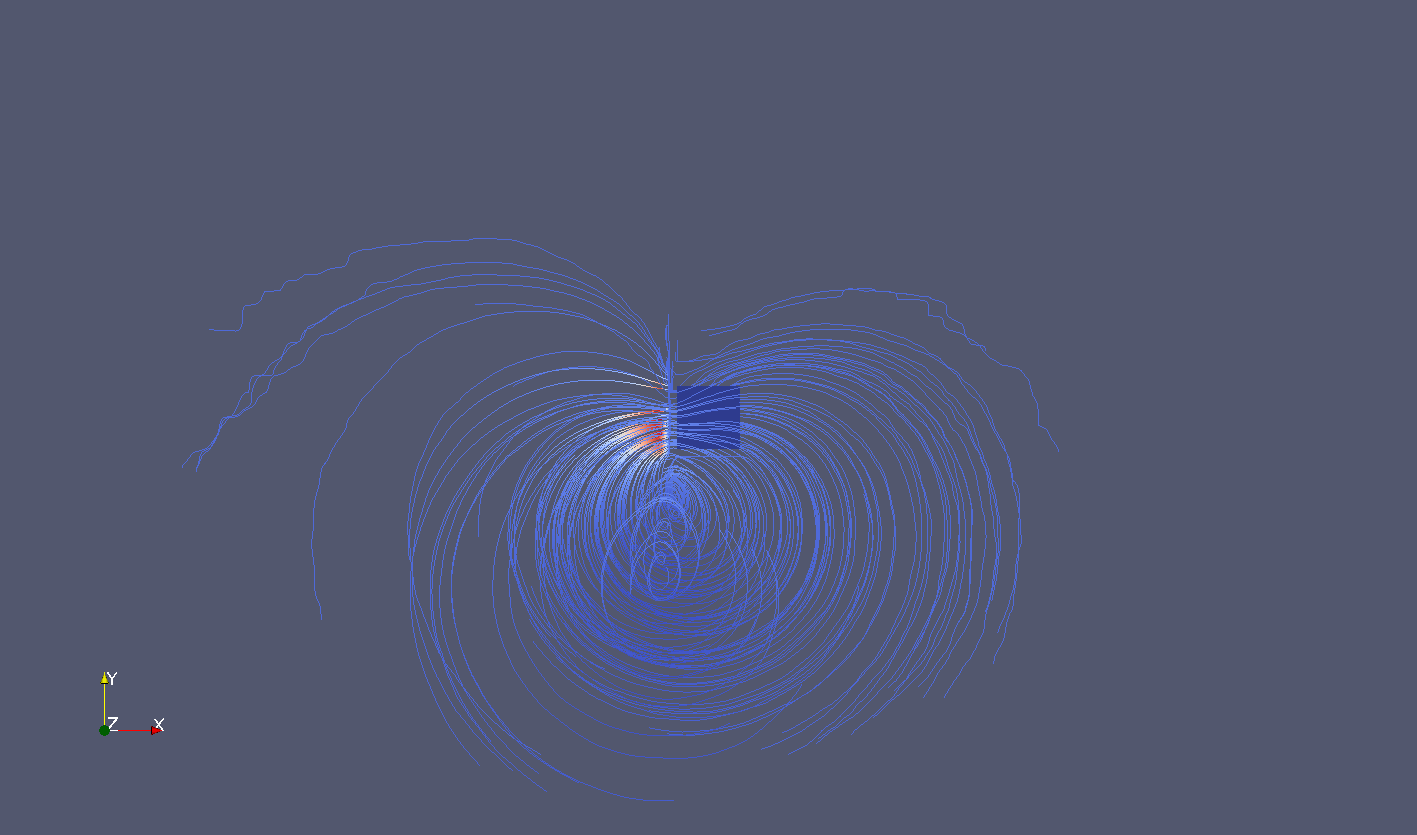
\includegraphics[width = 0.49 \textwidth]{images/case6_jph_paths}
		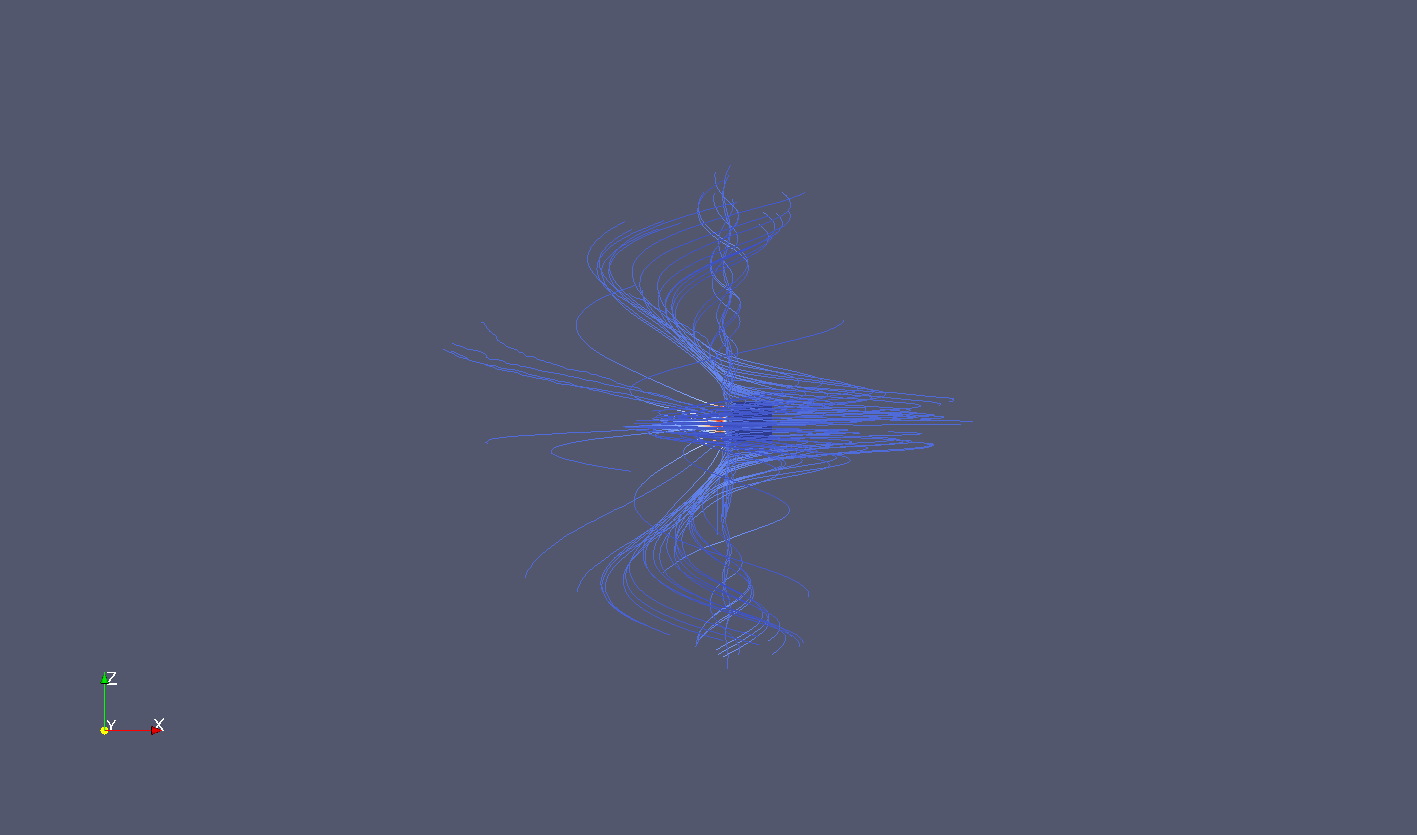
\includegraphics[width = 0.49 \textwidth]{images/case6_jph_paths_2}
		\caption{The trajectories of the electrons emmited by the photoelectric effect in simulation \(6\). It can be seen that some
		of the trajectories coincide with the volume occupied by the langmuir probes. The electrons are strongly affected by the magnetic
		field \(\vec{B}\), and follows a gyrating path.}
 	\end{figure}


\subsection{Potential difference with P-E and no P-E}

    \begin{figure}
        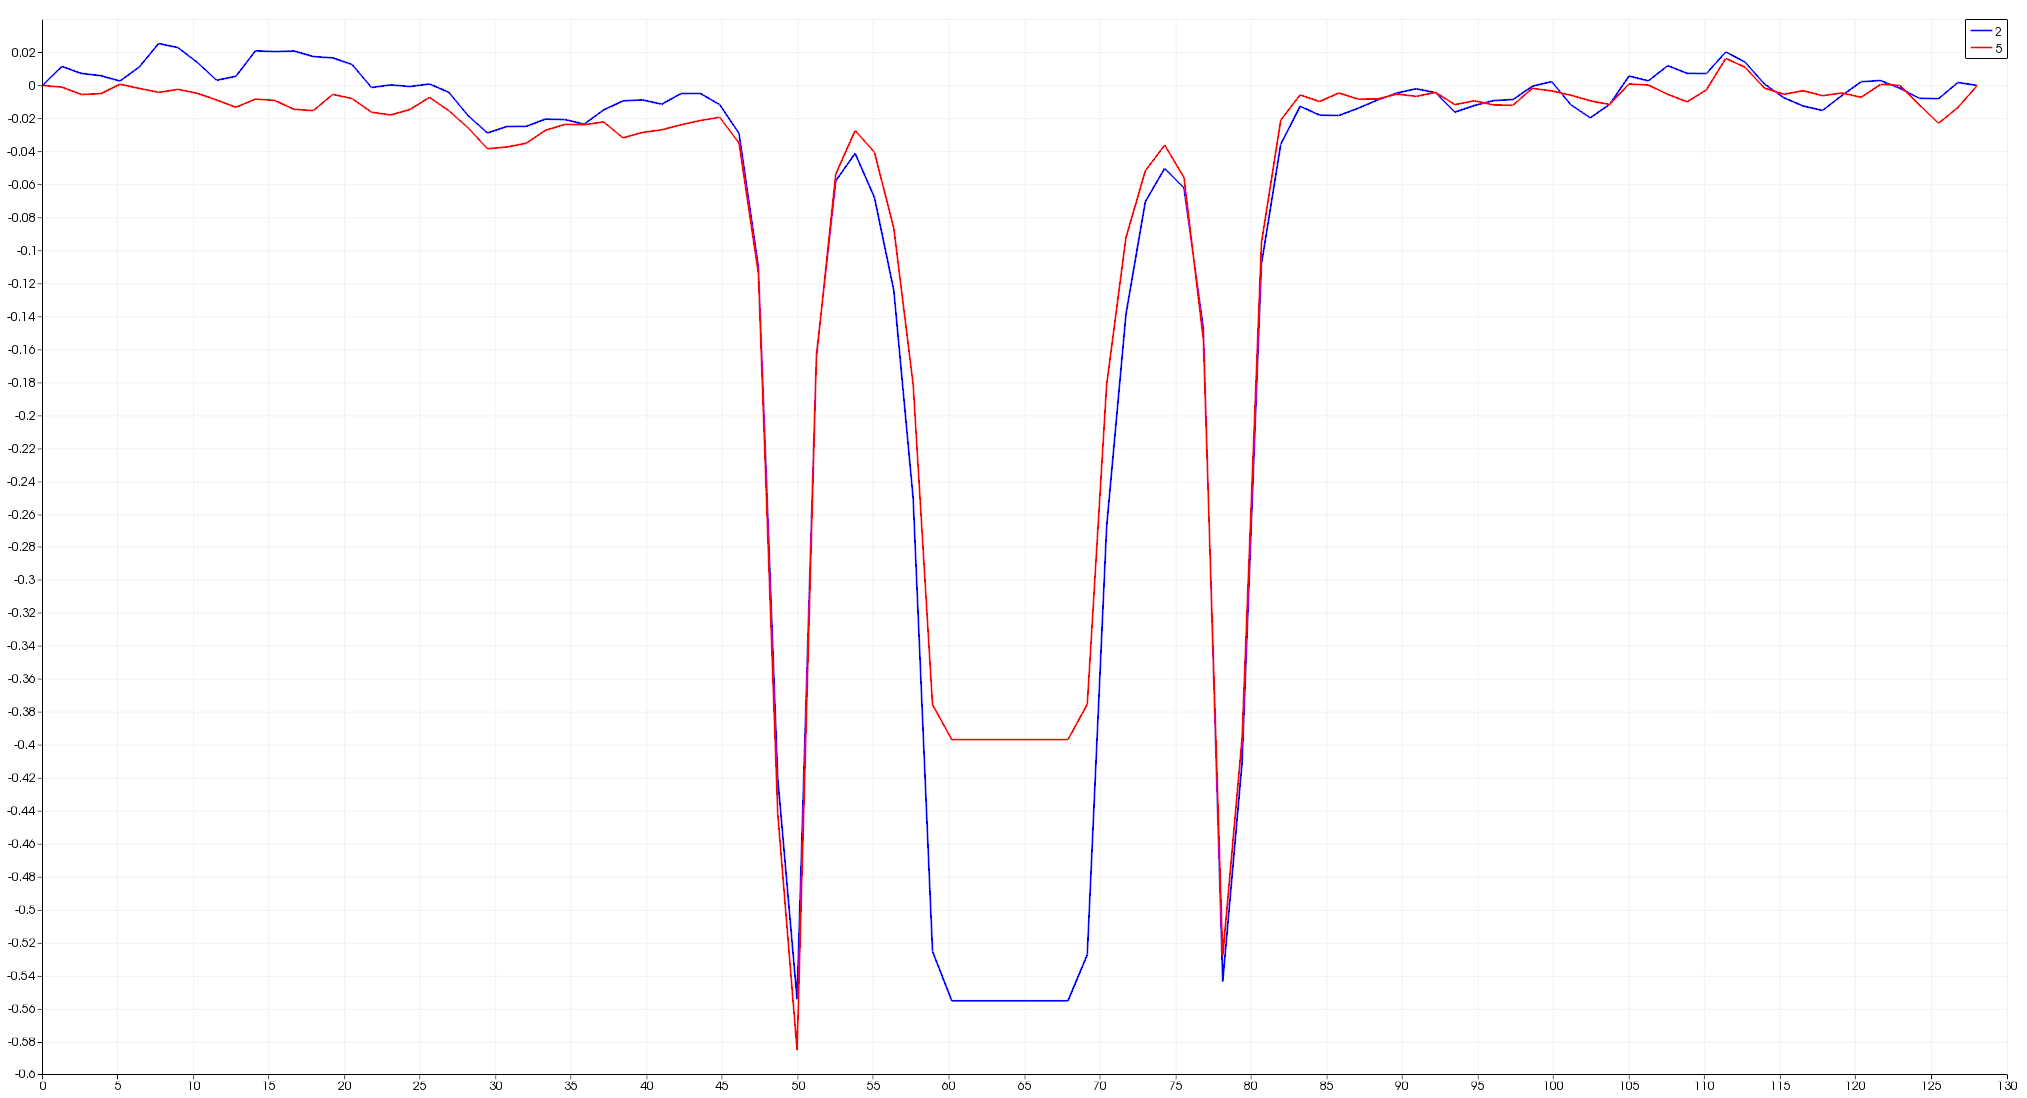
\includegraphics[width = 0.3 \textwidth]{images/pot_case25.png}
        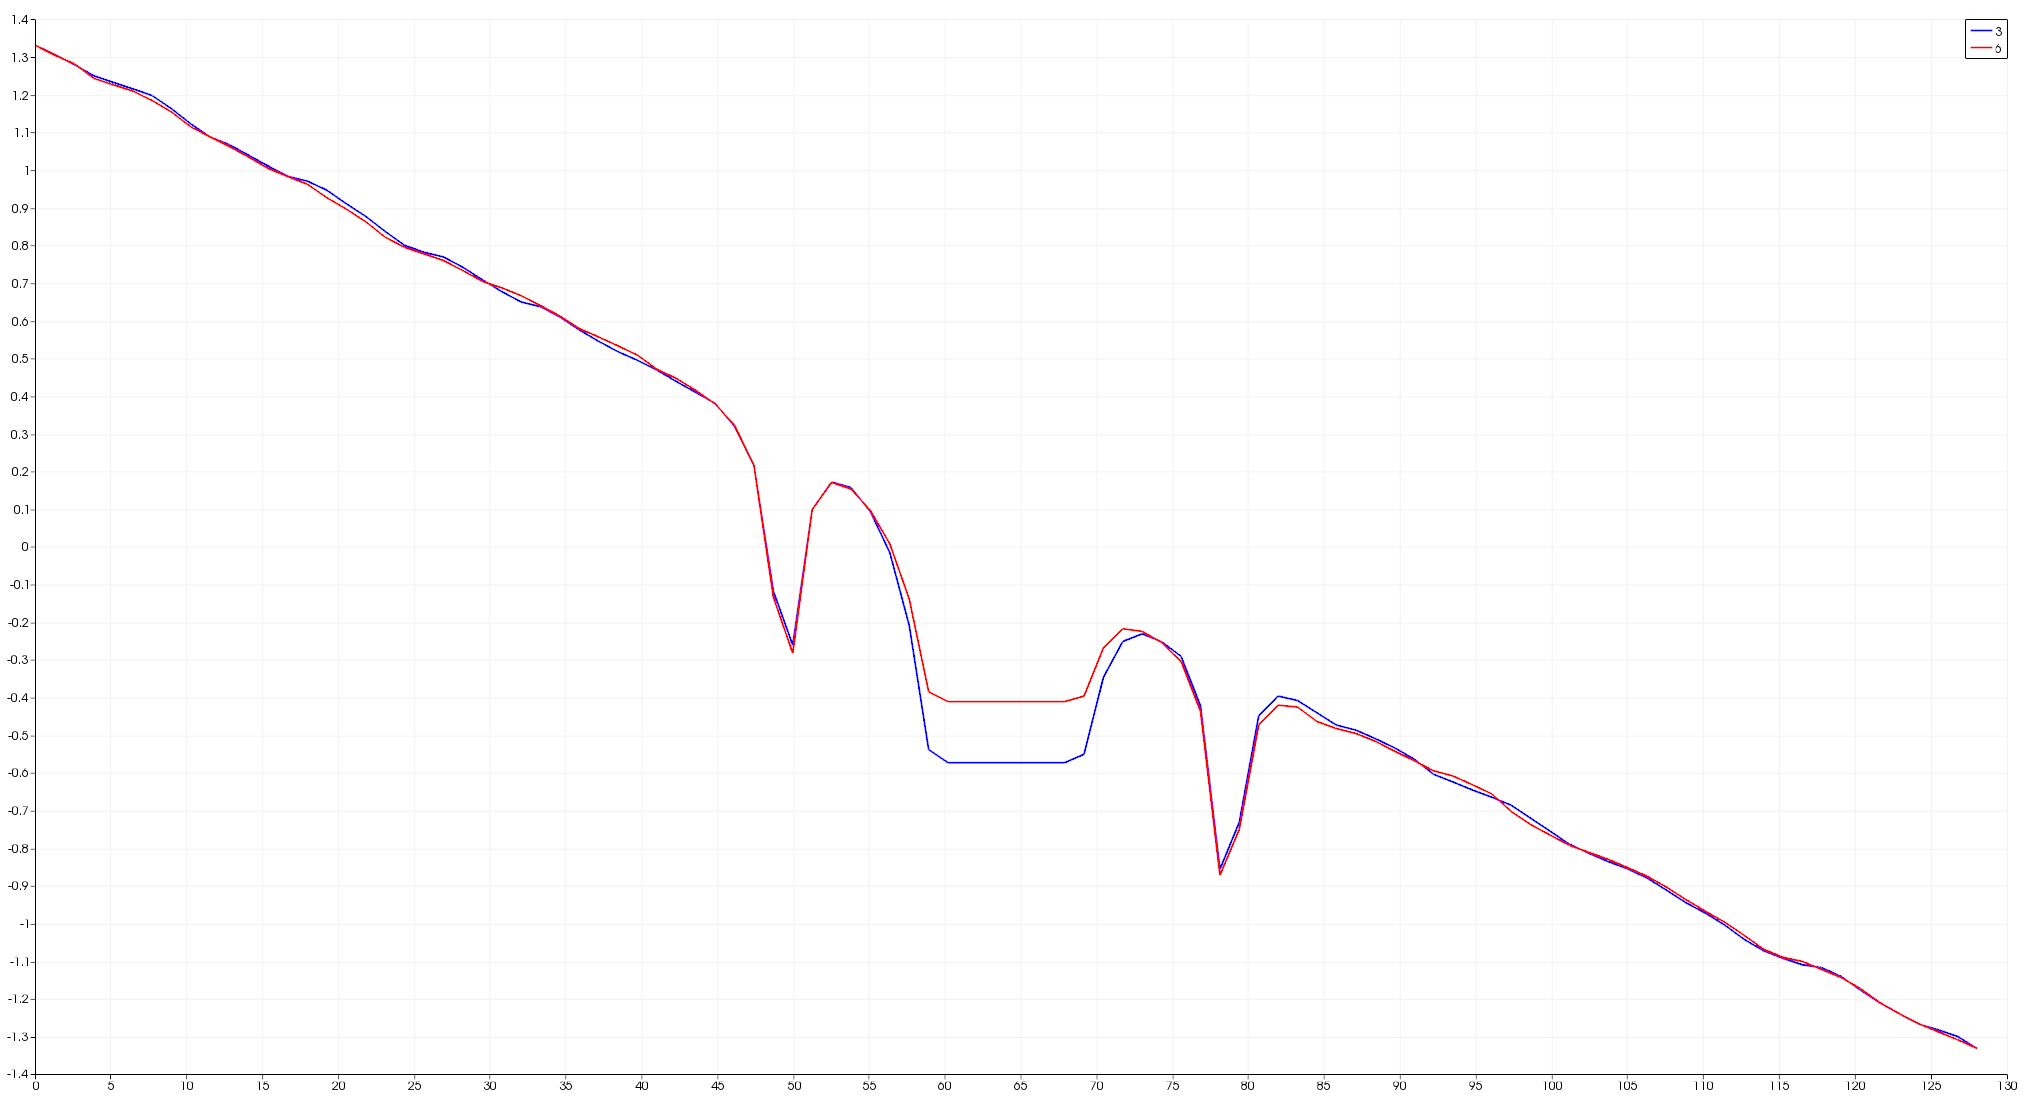
\includegraphics[width = 0.3 \textwidth]{images/pot_case36.png}
        \caption{Potential of spacecraft and surroundings with P-E and without P-E. Figure on the left displays difference between case 1 and 4. Middle figure displays difference between case 2 and 5. Rightmost figure displays difference between case 3 and 6.}
    \end{figure}



\subsection{Wake plots}

    \begin{figure}
        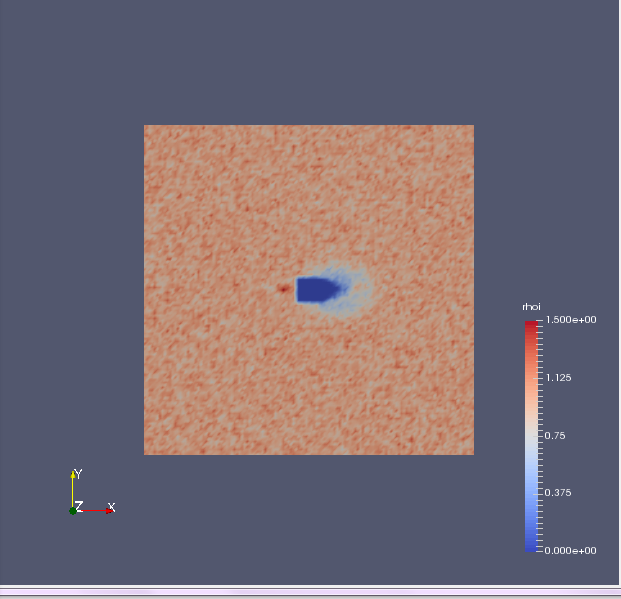
\includegraphics[width = 0.3 \textwidth]{images/ion density case1}
        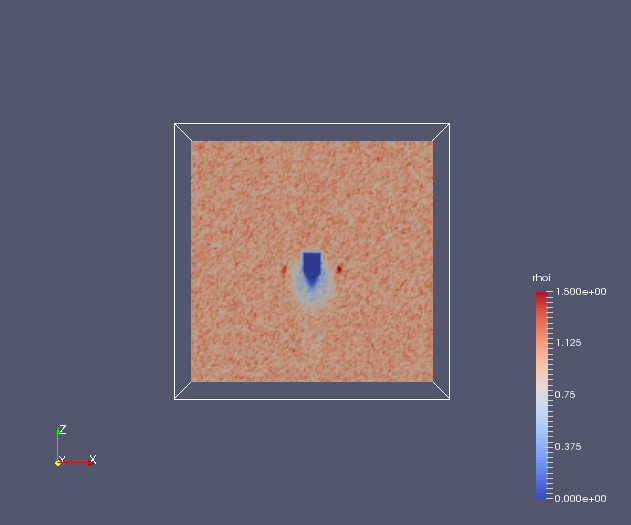
\includegraphics[width = 0.3 \textwidth]{images/ion density x-z case2}
	 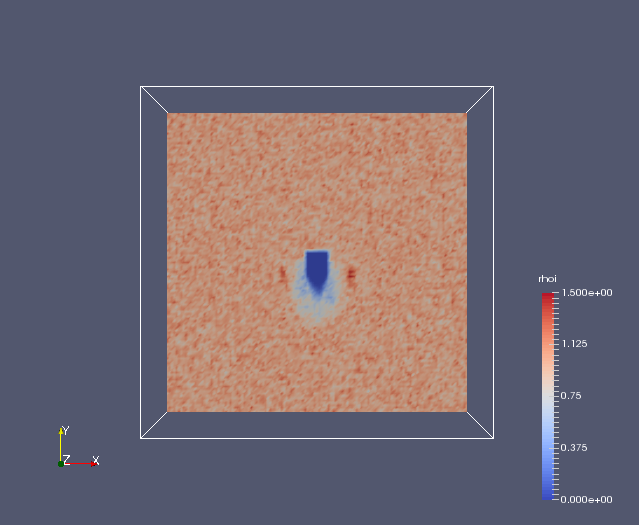
\includegraphics[width = 0.3 \textwidth]{images/ion density x-y case3}
        \caption{Ion density of spacecraft and surroundings without P-E. Figure on the left displays case 1. Middle figure displays case 2. Rightmost figure displays case 3.}
    \end{figure}
